% =====================================
% Section:Examples on Imaging modalities on SBRT
% =====================================

\label{sec:case2}


In the this section an exploration of common use of PET/CT for SBRT on the liver as well as the use of MRI its reviewed. The intention of this section is to ground the previous findings with some clincal examples.

\section*{Integrating respiratory-gated PET-based target volume delineation in liver SBRT planning}



\section*{Stereotactic MR-Guided Radiotherapy for Liver Metastases}

This study evaluates local treatment options for liver metastases, emphasizing the use of Stereotactic Body Radiation Therapy (SBRT). SBRT is a good choice for its ability to offer good local control and reduced toxicity levels, despite being a relatively novel application for liver conditions. Liver SBRT is a noninvasive technique that can be applied on an outpatient basis and is easy to combine sequentially with systemic treatments because of its excellent tolerance.

The study faced challenges previously established: liver metastases suffer from poor tissue contrast in X-ray imaging, complex anatomy requires advanced imaging, and breathing and diaphragm movement can prone to errors. The paper aims to solve this with the use of online cine MR sequences, MR Linac systems that combine gating (breath-hold treatments) and live tracking.

The authors reported a prospective registry covering treatments from October 2019 to April 2022. They treated 26 patients for 31 lesions using stereotactic MR-guided radiotherapy (MRgRT). According to their findings, nearly 90\% of the patients had been previously treated for one or more hepatic metastases, primarily through systemic treatment. Patient selection was conducted by a multidisciplinary tumor board and a technical board, assessing eligibility for MRgRT. The study included candidates with synchronous or metachronous oligo-metastatic liver metastases.

The researchers administered a radiation dose of 50 Gy in 5 fractions for 54.8\% of the lesions, with the dose increased to 60 Gy for 25\% of the lesions. They reported a median Planning Target Volume (PTV) of 35.6 cc, with a range from 9.9 to 343.2 cc. An adaptive protocol was implemented for 16.1\% of the lesions. Bordeau et al.~\cite{bordeau2023}. The study protocol involved patients undergoing both contrast-enhanced CT and 0.35T MRI simulations using the MRIdian® system. These simulations, when registered with enhanced 1.5T MRI, improve the precision and effectiveness of the Stereotactic Body Radiation Therapy (SBRT) planning.


\begin{figure}[ht]
	\centering
	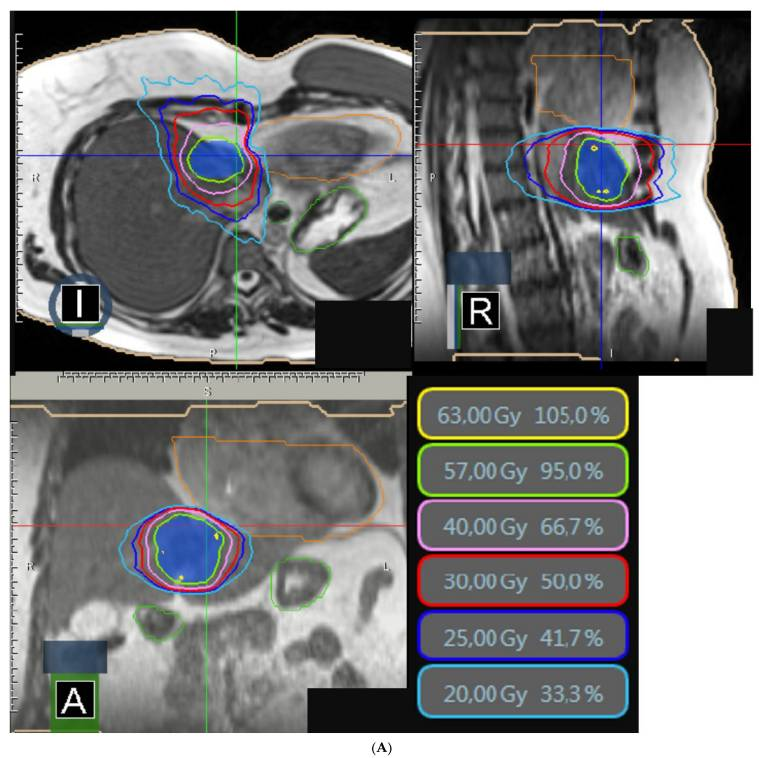
\includegraphics[width=0.5\textwidth]{assets/MRISBRT.jpeg}
	\caption{Dosimetry example for a liver metastasis from breast cancer. Planning Target Volume (PTV) shown in blue colorwash with isodose lines.}
	\label{fig:liver-metastasis-dosimetry}
\end{figure}

In their results, they included no MRgRT-related acute toxicities. However they reported gastrointestinal toxicity, and late toxicities that were related to metastatic disease progression. They confirmed the feasibility and good tolerance of the treatment in that indication. Acute and late gastrointestinal and liver toxicities were low and mostly unrelated to MRgRT, they added. OAR were accounted for and monitored. 
